

There are several ways to get dependencies as sources into your project. A relatively straightforward but dangerous way is to manually download or clone them into a subfolder inside your project and then add this folder with add\_subdirectory. While this works and is pretty fast, it quickly becomes tedious and hard to maintain. So, this should be automated as soon as possible.

\begin{tcolorbox}[colback=webgreen!5!white,colframe=webgreen!75!black,title=Note]
The practice of downloading and integrating a copy of a third-party software directly into a product is called vendoring. While it has the advantage that it often makes building software easy, it creates issues with packaging libraries. Vendoring is avoided by either using either a package manager or by installing the third-party software in a location on your system.
\end{tcolorbox}

\subsubsubsection{5.5.1\hspace{0.2cm}下载依赖项作为源代码}

At the base of getting external content is the CMake ExternalProject module and the more sophisticated FetchContent module, which is built on ExternalProject. While ExternalProject offers more flexibility, FetchContent is often more convenient to use, especially if the downloaded project is also built using CMake. Both of them download projects as source files and can be used to build them.

\hspace*{\fill} \\ %插入空行
\noindent
\textbf{使用FetchContent}

For external projects that use CMake to build, using the FetchContent module is the way of choice to add source dependencies. For binary dependencies, using find\_package and find modules is still the preferred way. One of the main differences between ExternalProject and FetchContent is that FetchContent downloads and configures external projects during configuration time, while ExternalProject does everything during the build step. The drawback to this is that the source and its configuration are not available during configuration time.

Before FetchContent, you would have used Git submodules to manually download the dependencies and then add them using add\_subdirectory. This works in some cases, but it can be rather inconvenient and cumbersome to maintain.

FetchContent provides a list of functions to pull in source dependencies, mainly FetchContent\_Declare, which defines the parameters for downloading and building FetchContent\_MakeAvailable, which populates the targets of the dependency and makes them available for the build. In the following example, the bertrand library for design by contract is pulled from Git using GitHub and made available for use:

\begin{lstlisting}[style=styleCMake]
include(FetchContent)
FetchContent_Declare(
	bertrand
	GIT_REPOSITORY https://github.com/bernedom/bertrand.git
	GIT_TAG 0.0.17)

FetchContent_MakeAvailable(bertrand)

add_executable(fetch_content_example)
target_link_libraries(
	fetch_content_example
	PRIVATE bertrand::bertrand
)
\end{lstlisting}

FetchContent\_MakeAvailable has been available since version 3.14, and it is recommended that you overpopulate the project manually by using FetchContent\_Populate. This should be used whenever possible because it makes code bases very maintainable due to its simplicity. As ExternalProject, FetchContent can download from HTTP(S), Git, SVN, Mercurial, and CVS, and the same good practices, such as specifying MD5 hashes for the downloaded content or using Git hashes, apply.

FetchContent\_MakeAvailable is the recommended way to make external CMake-based projects available, but if you want to have more control over your external projects, it is also possible to populate the projects manually. The following example does the same as the previous example but in a more verbose way:

\begin{lstlisting}[style=styleCMake]
FetchContent_Declare(
	bertrand
	GIT_REPOSITORY https://github.com/bernedom/bertrand.git
	GIT_TAG 0.0.17)
if(NOT bertrand_POPULATED)
FetchContent_Populate(bertrand)
add_subdirectory(${bertrand_SOURCE_DIR} ${bertrand_BINARY_DIR})
endif()
\end{lstlisting}

FetchContent\_Populate has additional options to be specified to control the build more closely. The signature is as follows:

\begin{lstlisting}[style=styleCMake]
FetchContent_Populate( <name>
	[QUIET]
	[SUBBUILD_DIR <subBuildDir>]
	[SOURCE_DIR <srcDir>]
	[BINARY_DIR <binDir>]
	...
)
\end{lstlisting}

Let's look at the options of FetchContent\_Populate:

\begin{itemize}
\item 
QUIET: This can be specified to suppress the output of the population if it succeeds. If the command fails, the output will be shown even if the option is specified to allow for debugging.

\item
SUBBUILD\_DIR: This specifies where the external project will be located. The default is \$\{CMAKE\_CURRENT\_BINARY\_DIR\}/<name>-subbuild. Generally, this option should be left as it is.

\item
SOURCE\_DIR and BINARY\_DIR: These change where the source and build directories of the external project are located. The default settings are \$\{CMAKE\_CURRENT\_BINARY\_DIR\}/<lcName>-src for SOURCE\_DIR and \$\{CMAKE\_CURRENT\_BINARY\_DIR\}/<lcName>-build for BINARY\_DIR.

\item
Any additional parameters added will be passed on to the underlying ExternalProject\_Add. However, FetchContent prohibits you from editing the commands for the different steps, so attempts to tamper with CONFIGURE\_COMMAND, BUILD\_COMMAND, INSTALL\_COMMAND, and TEST\_COMMAND will cause FetchContent\_Populate to fail with an error.
\end{itemize}

\begin{tcolorbox}[colback=webgreen!5!white,colframe=webgreen!75!black,title=Note]
If you find yourself in a situation where you need to pass options to the underlying ExternalProject\_Add, consider using ExternalProject directly instead of first going through FetchContent.
\end{tcolorbox}

Information about the source and build directories, along with whether a project has been populated, can be retrieved either by reading the <name>\_SOURCE\_DIR, <name>\_BINARY\_DIR, and <name>\_POPULATED variables or by calling FetchContent\_GetProperties. Note that <name> will always be available in all caps and all lowercase. This is so that CMake can identify the packages despite different capitalizations.
 
Another big advantage of FetchContent is that it can handle cases where the external projects share common dependencies and prevent them from being downloaded and built multiple times. The first time a dependency is defined over FetchContent the details are cached, and any further definitions will be silently ignored. The benefit of this is that a parent project can overrule the dependencies of the child projects.

Let's assume we have a top project called MyProject that fetches two external projects, Project\_A and Project\_B, with each depending on a third external project called AwesomeLib, but on a different minor version. In most cases, we do not want to download and use two versions of AwesomeLib but only one to avoid conflicts. The following diagram, shows what the dependency graph might look like:

\begin{center}
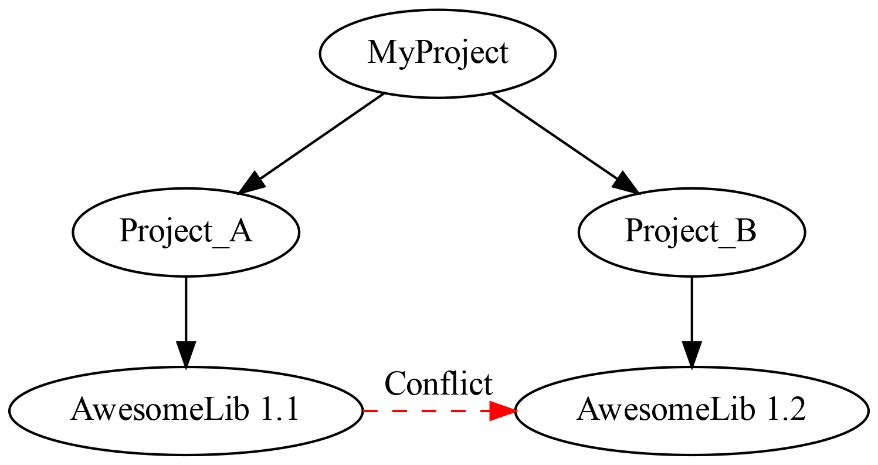
\includegraphics[width=0.6\textwidth]{content/2/chapter5/images/1.jpg}\\
Figure 5.1 – Both Project\_A and Project\_B depend on different versions of AwesomeLib
\end{center}

To resolve this, we can specify which version of AwesomeLib to pull by placing a FetchContent\_Declare call for AwesomeLib in the top-level CMakeLists.txt file. The order of the declaration inside the CMakeLists.txt file is not relevant here, only the level on which it is declared. Since both Project\_A and Project\_B contain the code to populate AwesomeLib, the top-level project does not need to use FetchContent\_MakeAvailable or FetchContent\_Populate. The resulting top-level CMakeLists.txt file might appear as follows:

\begin{lstlisting}[style=styleCMake]
include(FetchContent)
FetchContent_Declare(Project_A GIT_REPOSITORY ... GIT_TAG ...)
FetchContent_Declare(Project_B GIT_REPOSITORY ... GIT_TAG ...)
# Force AwesomeLib dependency to a certain version
FetchContent_Declare(AwesomeLib
GIT_REPOSITORY … GIT_TAG 1.2 )
FetchContent_MakeAvailable(Project_A)
FetchContent_MakeAvailable(Project_B)
\end{lstlisting}

This will force AwesomeLib to be pinned to version 1.2 for all projects. Of course, this only works if the interface between the versions required by Project\_A and Project\_B are compatible, resulting in a dependency graph, as illustrated in the following diagram:

\begin{center}
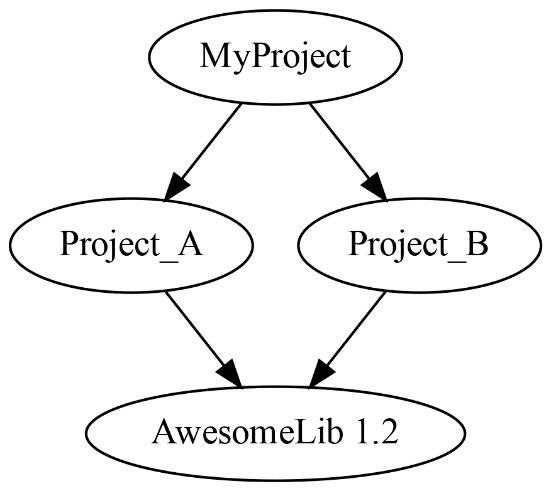
\includegraphics[width=0.5\textwidth]{content/2/chapter5/images/2.jpg}\\
Figure 5.2 – The corrected dependency graph after MyProject declares the version of AwesomeLib
\end{center}

Adding dependencies as sources has some advantages, but it comes with major drawbacks in that it increases configuration and build time considerably. In Chapter 9, Creating Reproducible Build Environments, we will tackle superbuilds with distributed repositories and provide more information about how to handle source dependencies.

At the beginning of the chapter, we looked at find\_package, which can be used to include binary dependencies, but we did not talk about how to conveniently download local binary dependencies using CMake. While FetchContent and ExternalProject can be used for that, it is not their purpose. Instead, dedicated package managers such as Conan and vcpkg will be better suited. Let's learn more about them next.

\hspace*{\fill} \\ %插入空行
\noindent
\textbf{使用ExternalProject}

The ExternalProject module is used to download and build external projects that are not fully integrated into the main project. When building an external project, the build is fully isolated, meaning that it will not automatically take over any settings regarding architecture or platforms. This isolation can come in handy to avoid clashes in the naming of targets or components. The external project creates a primary target and several child targets that contain the following isolated build steps:

\begin{enumerate}
\item 
Download: ExternalProject can download content in several ways, such as through pure HTTPS downloads or by accessing versioning systems such as Git, Subversion, Mercurial, and CVS. If the contents are archived, the download step will also unpack them.

\item 
Updating and patching: The downloaded source code can either be patched or updated to the newest version if the content is pulled from a Server Configuration Monitor (SCM).

\item 
Configure: If the downloaded source uses CMake, the configure step is executed on it. For non-CMake projects, a custom command that does the configuration can be provided.

\item 
Build: By default, the same build tool that is used in the main project is used to build the dependency, but a custom command can be provided if this is not desired. If a custom build command is supplied, it is up to the user to ensure that the necessary compiler flags are passed on so that the results are ABI-compatible.

\item 
Install: The isolated build can be installed locally, usually somewhere in the build tree of the main project.

\item 
Test: If the external content comes with a set of tests, the main project might choose to run them. By default, the tests are not run.
\end{enumerate}

All the steps, including downloading, run at build time. So, depending on the external project, this can increase the build time quite significantly. CMake caches the downloads and builds, so unless the external project has been changed, the overhead is primarily for the first run. The possibility of adding more steps to the external build does exist, but for most projects, the default steps are sufficient. The steps can be customized or omitted, as we will discover later.

In the following example, the bertrand library for using the design by contract is downloaded over HTTPS and locally installed in the current build directory:

\begin{lstlisting}[style=styleCMake]
include(ExternalProject)
ExternalProject_Add(
	bertrand
	URL https://github.com/bernedom/bertrand/archive
	/refs/tags/0.0.17.tar.gz
	URL_HASH MD5=354141c50b8707f2574b69f30cef0238
	INSTALL_DIR ${CMAKE_CURRENT_BINARY_DIR}/bertrand_install
	CMAKE_CACHE_ARGS -DBERTRAND_BUILD_TESTING:BOOL=OFF
	-DCMAKE_INSTALL_PREFIX:PATH=<INSTALL_DIR>
)
\end{lstlisting}

Note that the ExternalProject module is not available by default and has to be included in the first line with include(ExternalProject). As the external library is installed in the local build directory, the INSTALL\_DIR option is specified. Since bertrand itself is a CMake project, the installation directory is passed as <INSTALL\_DIR> by using the CMAKE\_INSTALL\_PREFIX variable to build the project. <INSTALL\_DIR> is a placeholder that points back to the INSTALL\_DIR option. ExternalProject knows placeholders for the various directories, such as <SOURCE\_DIR>, <BINARY\_DIR>, and <DOWNLOAD\_DIR>. For a complete list, please consult the module documentation at \url{https://cmake.org/cmake/help/latest/module/ExternalProject.html}. 

\begin{tcolorbox}[colback=blue!5!white,colframe=blue!75!black,title=Verify Your Downloads]
It is highly recommended that you add the download hash to any URL, as this sends you a notification if the contents of an artifact change.
\end{tcolorbox}

For this to work, any target that depends on bertrand has to be built after the external dependency. As bertrand is a header-only library, we want to add the include path to a target. Using the external project for another target in CMake could look similar to the following:

\begin{lstlisting}[style=styleCMake]
ExternalProject_Get_Property(bertrand INSTALL_DIR)
set(BERTRAND_DOWNLOADED_INSTALL_DIR "${INSTALL_DIR}")

# Create a target to build an executable
add_executable(external_project_example)
# make the executable to be built depend on the external
project
# to force downloading first
add_dependencies(external_project_example bertrand)

# make the header file for bertrand available
target_include_directories(external_project_example PRIVATE
${BERTRAND_DOWNLOADED_INSTALL_DIR}/include)
\end{lstlisting}

In the first line, the installation directory is retrieved with ExternalProject\_Get\_Property and stored in the INSTALL\_DIR variable. Unfortunately, the variable name is always the same as the property, so it is recommended that you store it immediately after retrieval in a variable with a unique name that expresses its use better.

Next, the target we want to build is created and made dependent on the target created by ExternalProject\_Add. This is necessary to enforce the correct build order.

And, finally, the path to the local installation is added to the target with target\_include\_directories. Additionally, we could import the CMake targets provided by the external library, but the purpose of this is to illustrate how this could work if the external project is not built by CMake.

Downloading from source code management systems happens with the respective options. For Git, this usually looks like the following:

\begin{lstlisting}[style=styleCMake]
ExternalProject_Add(MyProject GIT_REPOSITORY
	https://github.com/PacktPublishing/SomeRandomProject.git
		GIT_TAG 56cc1aaf50918f208e2ff2ef5e8ec0111097fb8d )
\end{lstlisting}

Note that GIT\_TAG can be any valid revision number for Git, including tag names and long and short hashes. If GIT\_TAG is omitted, the latest version of the default branch—usually called main or master—is downloaded. We highly recommend that you always specify the version to download. The most robust way is to define a commit hash, as tags can be moved around, although they rarely are in practice. Downloading from SVN is similar to downloading from Git. For additional details, please consult the official documentation for ExternalProject.

\hspace*{\fill} \\ %插入空行
\noindent
\textbf{处理非CMake项目和交叉编译}

A common use case for ExternalProject is to build dependencies that are not handled by CMake but by autotools or automake instead. In that case, you would need to specify the configuration and build commands as follows:

\begin{lstlisting}[style=styleCMake]
find_program(MAKE_EXECUTABLE NAMES nmake gmake make)
ExternalProject_Add(MyAutotoolsProject
	URL someUrl
	INSTALL_DIR ${CMAKE_CURRENT_BINARY_DIR}/myProject_install
	CONFIGURE_COMMAND <SOURCE_DIR>/configure --prefix=<INSTALL_DIR>
	BUILD_COMMAND ${MAKE_EXECUTABLE}
)
\end{lstlisting}

Note that the first find\_program command is used to find a version of make and store it in the MAKE\_EXECUTABLE variable. A common issue with external projects is that you have to closely control where the dependencies are installed. Most projects want to install to a default system location, which often requires root privileges and could accidentally pollute a system. So, passing the necessary options to the configuration or a build step is often necessary. Another way to handle this is to avoid the installation process entirely by replacing INSTALL\_COMMAND with an empty string as follows:

\begin{lstlisting}[style=styleCMake]
ExternalProject_Add(MyAutotoolsProject
	URL someUrl
	CONFIGURE_COMMAND <SOURCE_DIR>/configure
	BUILD_COMMAND ${MAKE_EXECUTABLE}
	INSTALL_COMMAND ""
)
\end{lstlisting}

One problem with using non-CMake projects such as this is that they do not define the necessary targets for using the dependency directly. So, in order to use an externally built library in another target, you often have to add the full library name to the target\_link\_libraries calls. The major drawback of this is that you have to manually maintain the different names and locations of the files for the various platforms. The find\_library or find\_file calls are of little use because they happen at configuration time, while ExternalProject only creates the necessary files at build time.

Another common use case is to use ExternalProject to build the contents of an existing source directory for a different target platform. In this case, the parameter that handles the downloading is simply omitted. If the external project is using CMake to build, the toolchain file can be passed as a CMake option to the external project. More information about toolchain files is available in Chapter 11, Automated Fuzzing with CMake. A very common pitfall here is that ExternalProject will not recognize any changes to the sources of the external projects, so CMake might not rebuild them. For this reason, the BUILD\_ALWAYS option should be passed, which has the downside of often making the build time considerably longer:

\begin{lstlisting}[style=styleCMake]
ExternalProject_Add(ProjectForADifferentPlatform
SOURCE_DIR 
	${CMAKE_CURRENT_LIST_DIR}/ProjectForADifferentPlatform
INSTALL_DIR ${CMAKE_CURRENT_BINARY_DIR}/
	ProjectForADifferentPlatform-install
CMAKE_ARGS
	-D CMAKE_TOOLCHAIN_FILE=${CMAKE_CURRENT_LIST_DIR}/fwtoolchain.cmake
	-D CMAKE_BUILD_TYPE=Release
	-D CMAKE_INSTALL_PREFIX=<INSTALL_DIR>
BUILD_ALWAYS YES
)
\end{lstlisting}

\hspace*{\fill} \\ %插入空行
\noindent
\textbf{管理ExternalProject中的步骤}

As mentioned in the preceding section, the steps of ExternalProject can be configured further and used in a more granular way. ExternalProject can be told to create regular targets for each step either by passing the STEP\_TARGETS option or by calling ExternalProject\_Add\_StepsTargets. The following calls expose both the configure step and the build step of an external project as targets:

\begin{lstlisting}[style=styleCMake]
ExternalProject_Add(MyProject
	# various options
	STEP_TARGETS configure build
)
ExternalProject_Add_StepTargets(MyProject configure build)
\end{lstlisting}

The targets are named after <mainName>-step. In the preceding example, two additional targets, MyProject-configure and MyProject-build, will be created. Creating step targets has two main uses: you are able to create custom steps that are sorted in the order of the download, configure, build, install, or test sequence, or you can make the steps dependent on other targets. These can either be regular targets, created by add\_executable, add\_library, or add\_custom\_target, or targets from other add executables. A common case is when external projects depend on each other, so the configuration step of one has to depend on another. In the next example, the configure step of project B will depend on the completion of project A:
 
\begin{lstlisting}[style=styleCMake]
ExternalProject_Add(ProjectA
	... # various options
		STEP_TARGETS install
)
ExternalProject_Add(ProjectB
... # various options
)
ExternalProject_Add_StepDependencies(ProjectB configure
	ProjectA)
\end{lstlisting}

Finally, we can also create custom steps to be interjected into an external project. The process of adding steps is done with the ExternalProject\_Add\_Step command. Custom steps cannot be named the same as any of the predefined steps (such as mkdir, download, update, patch, configure, build, install, or test). The following example will create a step that adds the license information of an external project to a specific tar file after building:

\begin{lstlisting}[style=styleCMake]
ExternalProject_Add_Step(bertrand_downloaded copy_license
	COMMAND ${CMAKE_COMMAND} -E tar "cvzf" ${CMAKE_CURRENT_
		BINARY_DIR}/licenses.tar.gz <SOURCE_DIR>/LICENSE
			DEPENDEES build
)
\end{lstlisting}

All in all, ExternalProject is a very powerful tool; however, it can become very complex to manage. Often, it is that flexibility that also makes ExternalProject hard to use. While it can help isolate builds, it often forces the project maintainer to manually expose any information from the inner workings of the external project to CMake, which, ironically, is what CMake is supposed to help with in the first place.











